\setcounter{dang}{1}
\begin{dang}{TÌM THAM SỐ ĐỂ HÀM SỐ CÓ CỰC TRỊ, CÓ CỰC TRỊ TẠI $x_0$}
\textbf{Loại 1. Tìm $m$ để hàm số có cực trị.}
\begin{enumerate}
\item \textit{Điều kiện để hàm số bậc 3 $y=ax^3+bx^2+cx+d$ ($a\neq 0$) có cực trị.}\\
Ta có $y'=3ax^2+2bx+c$.\\
Đồ thị hàm số có $2$ điểm cực trị khi phương trình $y'=0$ có hai nghiệm phân biệt $\Leftrightarrow b^2-3ac>0$.
\item \textit{Điều kiện để hàm số $f(x)=ax^4+bx^2+c(a\neq 0)$ có cực trị.}\\
Ta có $y'=4ax^3+2bx=2x(2ax^2+b)$\\
\textbf{\textit{Trường hợp 1.}} $ab \ge 0$. Khi đó $f'(x)$ có nghiệm duy nhất $x=0$ và $f'(x)$ đổi dấu đúng một lần khi đi qua $x=0$. Do đó $f(x)$ chỉ có đúng một điểm cực trị.\\
\textbf{\textit{Trường hợp 2.}} $ab<0$. Khi đó $f'(x)$ có ba nghiệm phân biệt và $f'(x)$ đổi dấu liên tiếp khi $x$ đi qua ba nghiệm này. Do đó $f(x)$ có ba điểm cực trị.
\end{enumerate}
% \textbf{\textit{Một số công thức áp dụng giải toán cực trị hàm số $f(x)=ax^4+bx^2+c$ $(a\neq 0)$.}}
% \begin{itemize}
% \item $f$ có một cực trị $\Leftrightarrow ab\geq 0$.\\
% \item $f$ có ba cực trị $\Leftrightarrow ab<0$.\\
% \item $f$ có đúng một cực trị và cực trị là cực tiểu $\Leftrightarrow\heva{&a>0\\&b\geq 0.}$ \\
% \item $f$ có đúng một cực trị và cực trị là cực đại $\Leftrightarrow\heva{&a<0\\&b\leq 0.}$ \\
% \item $f$ có hai cực tiểu và một cực đại $\Leftrightarrow\heva{&a>0\\&b<0.}$ \\
% \item $f$ có một cực tiểu và hai cực đại $\Leftrightarrow\heva{&a<0\\&b>0.}$ \\
% \item $f$ có ba cực trị $\Leftrightarrow ab<0$.\\
% Khi đó $y'=0\Leftrightarrow\hoac{&x=0\\&x=\pm\sqrt{\dfrac{-b}{2a}}.}$ \\
% Với $x=0\Rightarrow y=c$ và $x=\pm\sqrt{\dfrac{-b}{2a}}\Rightarrow y=\dfrac{ab^2}{4a^2}-\dfrac{b^2}{2a}+c=\dfrac{-b^2+4ac}{4a}=-\dfrac{\Delta}{4a}$ với $\Delta=b^2-4ac$.\\
% Vậy đồ thị hàm số có ba điểm cực trị là $A(0;c)$, $B\left(-\sqrt{-\dfrac{b}{2a}};-\dfrac{\Delta}{4a}\right)$, $C\left(\sqrt{-\dfrac{b}{2a}};-\dfrac{\Delta}{4a}\right)$.\\
% Tính được $AB=AC=\sqrt{\dfrac{b^4}{16a^2}-\dfrac{b}{2a}}$; $BC=2\sqrt{-\dfrac{b}{2a}}$.
% \end{itemize}


\textbf{Loại 2. Tìm $m$ để hàm số đạt cực trị tại $x_0$.} \\
\textbf{\underline{Bài toán}.} Tìm tham số để hàm số $y=f(x)$ đạt cực trị tại điểm $x=x_0$?\\
\textbf{\underline{Phương pháp}:}
\begin{enumerate}[\bf Bước 1.]
\item Tìm tập xác định $\mathscr{D}$. Tính đạo hàm $y'$ và $y''$.
\item Dựa vào nội dung định lí 3. \\
Giả sử $y=f(x)$ có đạo hàm cấp $2$ trong khoảng $\left(x_0-h;x_0+h\right)$, với $h>0$.\\
Nếu $y'\left(x_0\right)=0$, $y''\left(x_0\right)>0$ thì $x_0$ là điểm cực tiểu.\\
Nếu $y'\left(x_0\right)=0$, $y''\left(x_0\right)<0$ thì $x_0$ là điểm cực đại.\\
Nếu $y'(x_0)=0$, $y''(x_0)=0$ thì cần xét dấu $y'$ theo $m$.
\item Với $m$ vừa tìm, thế vào hàm số và thử lại.
\end{enumerate}
\begin{note}
Nếu đề bài yêu cầu tìm giá trị cực trị tương ứng, ta sẽ thế $x=x_0$, $m=?$ vào $y=f(x)$.
\end{note}
\end{dang}
\paragraph{Các ví dụ}
\begin{vd}%Câu 1.%[2D1B2-5]
	Tìm tham số $m$ để các hàm số
\begin{enumerate}
	\item[a)] $y=x^3-3x^2+(m-1)x+2$ có cực trị.
	\item[b)] $y=\dfrac{1}{3}(m-1)x^3+(m-2)x^2-4x+1$ không có cực trị.
	\item[c)] $y=-x^4+2(2m-1)x^2+3$ có đúng $1$ cực trị.
	\item[d)] $y=x^4+2\left(m^2-1\right)x^2+1$ có $3$ điểm cực trị.
	\item[e)] $y=mx^4+\left(m^2-9\right)x^2+1$ có $2$ điểm cực đại và $1$ điểm cực tiểu.
	\item[f)] $y=mx^4+(2m-1)x^2+m-2$ chỉ có cực đại và không có cực tiểu.
\end{enumerate}
\loigiai
{
\begin{enumerate}
	\item[a)] $y'=3x^2-6x+m-1$.\\
Hàm số có cực trị $\Leftrightarrow$ hàm số có hai điểm cực trị $\Leftrightarrow$ $y'=0$ có hai nghiệm phân biệt \\
$\Leftrightarrow$ $9-3(m-1)>0\Leftrightarrow m<4$.
\item[b)] $y'=(m-1)x^2+2(m-2)x-4$.\\
Trường hợp 1. $m-1=0\Leftrightarrow m=1$. \\
Khi đó, $y'=-2x-4=0\Leftrightarrow x=-2$.\\
Ta có $y'$ là nhị thức nhậc nhất nên $y'$ đổi dấu khi $x$ qua $x=-2$.\\
Vậy hàm số có cực trị, suy ra loại $m=1$.\\
Trường hợp 2. $m-1\neq0\Leftrightarrow m\neq1$. \\
Hàm số không có cực trị $\Leftrightarrow$ $y'=0$ vô nghiệm hoặc có nghiệm kép $\Leftrightarrow$ $\left(m-2\right)^2+4(m-1)\leq0\Leftrightarrow m^2\leq0\Leftrightarrow m=0$.\\
Vậy $m=0$.
\item[c)] $y'=-4x^3+4(2m-1)x$. \\
Hàm số có đúng $1$ cực trị $\Leftrightarrow$ $-16(2m-1)\geq0\Leftrightarrow m\leq\dfrac{1}{2}$.
\item[d)] $y'=4x^3+4\left(m^2-1\right)x$. \\
Hàm số có $3$ điểm cực trị $\Leftrightarrow$ $16\left(m^2-1\right)<0\Leftrightarrow -1<m<1$.
\item[e)] $y'=4mx^3+2\left(m^2-9\right)$. \\
Hàm số có $2$ điểm cực đại và $1$ điểm cực tiểu
\[\Leftrightarrow\heva{&4m<0\\&8m\left(m^2-9\right)<0}\Leftrightarrow\heva{&m<0\\&m^2-9>0}\Leftrightarrow\heva{&m<0\\&\hoac{&m>3\\&m<-3}}\Leftrightarrow m<-3.\]
\item[f)] $y'=4mx^3+2(2m-1)x$. \\
Trường hợp 1. $m=0$. \\
Khi đó, $y=-x^2-2$ và $y'=-2x$. \\
Ta có $y'=0\Leftrightarrow x=0$. \\
Bảng biến thiên của hàm số
\begin{center}
\begin{tikzpicture}[scale=1]
\tkzTabInit[nocadre=false, lgt=1.2, espcl=2.5, deltacl=0.6]{$x$/0.6, $y'$/0.6, $y$/2}{$-\infty$, $0$, $+\infty$}
\tkzTabLine{,+,0,-,}
\tkzTabVar{-/$-\infty$, +/$-2$, -/$-\infty$}
\end{tikzpicture}
\end{center}
Từ bảng biến thiên ta thấy hàm số có cực đại và không có cực tiểu, suy ra $m=0$ thỏa mãn. \\
Trường hợp 2. $m\neq0$. \\
Hàm số có cực đại và không có cực tiểu
\[\Leftrightarrow\heva{&4m<0\\&8m(2m-1)\geq0}\Leftrightarrow\heva{&m<0\\&2m-1\leq0}\Leftrightarrow\heva{&m<0\\&m\leq\dfrac{1}{2}}\Leftrightarrow m<0.\]
\end{enumerate}
}
%<MyLT>
\end{vd}

\begin{vd}%[Thành Đức Trung]%[2D1B2-3]%Câu 1.
	Tìm tham số $m$ để các hàm số
	\begin{enumerate}
		\item[a)] $y=x^3-(m-1)x+1$ đạt cực tiểu tại $x=2$.
		\item[b)] $y=\dfrac{1}{3}x^3-mx^2+\left(m^2-m+1\right)x+1$ đạt cực đại tại $x=1$.
		\item[c)] $y=\dfrac{1}{4}(m-1)x^4$ đạt cực đại tại $x=0$.
		\item[d)] $y=-x^4+2(m-2)x^2+m-3$ đạt cực đại tại $x=0$.
		\item[e)] $y=x^4-2mx^2+2m+m^4-5$ đạt cực tiểu tại $x=-1$.
	\end{enumerate}
\loigiai
{
\begin{enumerate}
\item[a)] $y'=3x^2-m+1$. \\
Hàm số đạt cực tiểu tại $x=2\Rightarrow y'(2)=0 \Leftrightarrow m=13$. \\
Với $m=13$, ta có $y'=3x^2-12$. \\
Ta có $y'=0\Leftrightarrow\hoac{&x=2\\&x=-2.}$.\\
Bảng xét dấu của đạo hàm
\begin{center}
\begin{tikzpicture}[scale=1]
\tkzTabInit[nocadre=false, lgt=1.2, espcl=2.5, deltacl=0.6]{$x$/0.6, $y'$/0.6}{$-\infty$, $-2$, $2$, $+\infty$}
\tkzTabLine{,+,0,-,0,+,}
\end{tikzpicture}
\end{center}
Từ bảng xét dấu ta có $x=2$ là điểm cực tiểu của hàm số.\\
Vậy $m=13$.
\item[b)] $y'=x^2-2mx+m^2-m+1$. \\
Hàm số đạt cực đại tại $x=1\Rightarrow y'(1)=0\Leftrightarrow m^2-3m+2=0\Leftrightarrow\hoac{&m=1\\&m=2.}$\\
Với $m=1$, ta có $y'=x^2-2x+1=\left(x-1\right)^2\geq0$. \\
Suy ra hàm số đồng biến, suy ra không có cực trị, loại $m=1$. \\
Với $m=2$, ta có $y'=x^2-4x+3$. \\
Ta có $y'=0\Leftrightarrow\hoac{&x=1\\&x=3.}$\\
Bảng xét dấu của đạo hàm
\begin{center}
\begin{tikzpicture}[scale=1]
\tkzTabInit[nocadre=false, lgt=1.2, espcl=2.5, deltacl=0.6]{$x$/0.6, $y'$/0.6}{$-\infty$, $1$, $3$, $+\infty$}
\tkzTabLine{,+,0,-,0,+,}
\end{tikzpicture}
\end{center}
Từ bảng xét dấu ta có $x=1$ là điểm cực đại của hàm số.\\
Vậy $m=2$.
\item[c)] $y'=4(m-1)x^3$. \\
Với $m=1$, ta có $y=0$, $\forall x\in\mathbb{R}$. \\
Khi đó $y$ là hàm hằng, suy ra hàm số không có cực trị, loại $m=1$. \\
Với $m<1$, ta có $y'=0\Leftrightarrow x=0$. \\
Bảng xét dấu của đạo hàm
\begin{center}
\begin{tikzpicture}[scale=1]
\tkzTabInit[nocadre=false, lgt=1.2, espcl=2.5, deltacl=0.6]{$x$/0.6, $y'$/0.6}{$-\infty$, $0$, $+\infty$}
\tkzTabLine{,+,0,-,}
\end{tikzpicture}
\end{center}
Từ bảng xét dấu ta có $x=0$ là điểm cực đại của hàm số, suy ra $m<1$: thỏa mãn. \\
Với $m>1$, ta có $y'=0\Leftrightarrow x=0$. \\
Bảng xét dấu của đạo hàm
\begin{center}
\begin{tikzpicture}[scale=1]
\tkzTabInit[nocadre=false, lgt=1.2, espcl=2.5, deltacl=0.6]{$x$/0.6, $y'$/0.6}{$-\infty$, $0$, $+\infty$}
\tkzTabLine{,-,0,+,}
\end{tikzpicture}
\end{center}
Từ bảng xét dấu ta có $x=0$ là điểm cực tiểu của hàm số, suy ra $m>1$: loại. \\
Vậy $m<1$.
\item[d)] $y'=-4x^3+4(m-2)x=-4x\left(x^2-(m-2)\right)$. \\
Ta có $y'=0\Leftrightarrow\hoac{&x=0\\&x^2=m-2.}$ \\
Với $m-2\leq0\Leftrightarrow m\leq2$, ta có $y'=0\Leftrightarrow x=0$. \\
Bảng xét dấu của đạo hàm
\begin{center}
\begin{tikzpicture}[scale=1]
\tkzTabInit[nocadre=false, lgt=1.2, espcl=2.5, deltacl=0.6]{$x$/0.6, $y'$/0.6}{$-\infty$, $0$, $+\infty$}
\tkzTabLine{,+,0,-,}
\end{tikzpicture}
\end{center}
Từ bảng xét dấu ta có $x=0$ là điểm cực đại của hàm số, suy ra $m\leq2$: thỏa mãn. \\
Với $m-2>0\Leftrightarrow m>2$, ta có $y'=0\Leftrightarrow\hoac{&x=0\\&x=\sqrt{m-2}\\&x=-\sqrt{m-2}.}$ \\
Bảng xét dấu của đạo hàm
\begin{center}
\begin{tikzpicture}[scale=1]
\tkzTabInit[nocadre=false, lgt=1.2, espcl=2.5, deltacl=0.6]{$x$/0.6, $y'$/0.6}{$-\infty$, $-\sqrt{m-2}$, $0$, $\sqrt{m-2}$, $+\infty$}
\tkzTabLine{,+,0,-,0,+,0,-,}
\end{tikzpicture}
\end{center}
Từ bảng xét dấu ta có $x=0$ là điểm cực tiểu của hàm số, suy ra $m>2$: loại. \\
Vậy $m\leq2$.
\item[e)] $y'=4x^3-4mx$. \\
Hàm số đạt cực tiểu tại $x=-1\Rightarrow y'(-1)=0\Leftrightarrow m=1$. \\
Với $m=1$, ta có $y'=4x^3-4x=4x\left(x^2-1\right)=0\Leftrightarrow\hoac{&x=0\\&x=1\\&x=-1.}$ \\
Bảng xét dấu của đạo hàm
\begin{center}
\begin{tikzpicture}[scale=1]
\tkzTabInit[nocadre=false, lgt=1.2, espcl=2.5, deltacl=0.6]{$x$/0.6, $y'$/0.6}{$-\infty$, $-1$, $0$, $1$, $+\infty$}
\tkzTabLine{,-,0,+,0,-,0,+,}
\end{tikzpicture}
\end{center}
Từ bảng xét dấu ta có $x=-1$ là điểm cực tiểu của hàm số, suy ra $m=1$: thỏa mãn. \\
Vậy $m=1$.
\end{enumerate}
}
\end{vd}

\paragraph{Các câu hỏi trắc nghiệm}
\Opensolutionfile{ans}[ans/BAI-2-DANG-2-GV]
\begin{ex}%Câu 2.%[2D1B2-4]
	Hàm số $y=x^3+mx+2$ có cả cực đại và cực tiểu khi 
	\choice
	{\True $m<0$}
	{$m>0$}
	{$m\geq 0$}
	{$m\leq 0$}
	\loigiai{
		$y'=3x^2+m$. Hàm số $y=x^3+mx+2$ có cả cực đại và cực tiểu khi và chỉ khi $y'=0$ có hai nghiệm phân biệt. Vậy $m<0$.}
%<MyLT>
\end{ex}

\begin{ex}%Câu 3.%[2D1B2-4]
	Cho hàm số $y=(m-2)x^3-mx-2$. Với giá trị nào của $m$ thì hàm số có cực trị?
	\choice
	{$0<m<2$}
	{$m<1$}
	{\True $m>2\vee m<0$}
	{$m>1$}
	\loigiai{
		Tập xác định $\mathscr{D}=\mathbb{R}$.\\
		Ta có $y'=3(m-2)x^2-m$.\\
		Cho $y'=0\Leftrightarrow 3(m-2)x^2-m=0$ $(1)$.
\begin{itemize}
		\item TH1: Xét $m=2\Rightarrow y'=-2<0$, $\forall x\in\mathbb{R}$ nên hàm số đã cho không có cực trị.\\
		\item TH2: Xét $m\neq 2$. \\
Hàm số có cực trị khi $\Delta'>0\Leftrightarrow m(m-2)>0\Leftrightarrow\hoac{&m>2\\&m<0.}$
\end{itemize}
		Vậy $m>2$ hoặc $m<0$.}
%<MyLT>
\end{ex}

\begin{ex}%Câu 4.%[2D1B2-4]
	Tìm tất cả tham số thực của $m$ để hàm số $y=\dfrac{1}{3}(m+2)x^3+x^2+\dfrac{1}{3}mx-2$ có cực đại, cực tiểu. 
	\choice
	{\True $m\in(-3;-2)\cup(-2;1)$}
	{$m\in(-3;1)$}
	{$m\in(-\infty;-3)\cup(1;+\infty)$}
	{$m\in(-2;1)$}
	\loigiai{
		$y'=(m+2)x^2+2x+\dfrac{1}{3}m$.\\
		Hàm số có cực đại, cực tiểu khi phương trình $y'=0$ có hai nghiệm phân biệt 
\[\Leftrightarrow\heva{&\Delta'>0\\&m+2\neq 0}\Leftrightarrow\heva{&1-\dfrac{1}{3}m^2-\dfrac{2}{3}m>0\\&m\neq-2}\Leftrightarrow\heva{&-3<m<1\\&m\neq-2}\Leftrightarrow\hoac{&-3<m <-2\\&-2<m<1.}\]
}
%<MyLT>
\end{ex}

\begin{ex}%Câu 5.%[2D1B2-4]
	Xác định các giá trị của tham số $m$ để đồ thị hàm số $y=mx^4-m^2x^2+2016$ có $3$ điểm cực trị?
	\choice
	{$m<0$}
	{\True $m>0$}
	{$\forall m\in\mathbb{R}\setminus\{0\}$}
	{Không tồn tại giá trị của $m$}
	\loigiai{
		Tập xác định $\mathscr{D}=\mathbb{R}$.\\
		Ta có $y'=4mx^3-2xm^2$.\\
		Để hàm số có $3$ điểm cực trị khi $\heva{&a\neq 0\\&a\cdot b<0}\Leftrightarrow\heva{&m\neq 0\\&-8m^3<0}\Leftrightarrow m>0$.}
%<MyLT>
\end{ex}
%%==========Câu 1
\begin{ex}%[Thành Đức Trung]%[2D1Y2-7]
	Hàm số $y=ax^3+bx^2+cx+d$ $(a\neq 0)$ có cực trị khi
	\choice
	{$y'=0$ vô nghiệm}
	{$y'=0$ có duy nhất một nghiệm}
	{$y'=0$ có nghiệm}
	{\True $y'=0$ có 2 nghiệm phân biệt}
\loigiai
{
}
\end{ex}
%%==========Câu 2
\begin{ex}%[Thành Đức Trung]%[2D1Y2-7]
	Hàm số $y=ax^3+bx^2+cx+d$ $(a\neq 0)$ có cực đại, cực tiểu khi
	\choice
	{$y'=0$ vô nghiệm}
	{$y'=0$ có duy nhất một nghiệm}
	{$y'=0$ có nghiệm}
	{\True $y'=0$ có 2 nghiệm phân biệt}
\loigiai
{
}
\end{ex}
%%==========Câu 3
\begin{ex}%[Thành Đức Trung]%[2D1B2-7]
	Hàm số $y=ax^3+bx^2+cx+d$ $(a\neq 0)$ có cực đại, cực tiểu và $x_{\text{CĐ}}<x_{\text{CT}}$ khi
	\choice
	{$y'=0$ có nghiệm, $a>0$}
	{\True $y'=0$ có hai nghiệm phân biệt, $a>0$}
	{$y'=0$ có nghiệm, $a<0$}
	{$y'=0$ có hai nghiệm phân biệt, $a<0$}
\loigiai
{
}
\end{ex}
%%==========Câu 4
\begin{ex}%[Thành Đức Trung]%[2D1B2-7]
	Hàm số $y=ax^3+bx^2+cx+d$ $(a\neq 0)$ có cực đại, cực tiểu và $x_{\text{CĐ}}>x_{\text{CT}}$ khi
	\choice
	{$y'=0$ có nghiệm, $a>0$}
	{$y'=0$ có hai nghiệm phân biệt, $a>0$}
	{$y'=0$ có nghiệm, $a<0$}
	{\True $y'=0$ có hai nghiệm phân biệt, $a<0$}
\loigiai
{
}
\end{ex}
%%==========Câu 5
\begin{ex}%[Thành Đức Trung]%[2D1Y2-7]
	Hàm số $y=ax^4+bx^2+c$ $(a\neq 0)$ có $3$ điểm cực trị khi và chỉ khi
	\choice
	{$b<0$}
	{$ab>0$}
	{$ab\leq 0$}
	{\True $ab<0$}
\loigiai
{
}
\end{ex}
%%==========Câu 6
\begin{ex}%[Thành Đức Trung]%[2D1Y2-7]
	Hàm số $y=ax^4+bx^2+c$ $(a\neq 0)$ có $1$ điểm cực trị khi và chỉ khi
	\choice
	{$b>0$}
	{\True $ab\geq 0$}
	{$ab<0$}
	{$b\leq 0$}
\loigiai
{
}
\end{ex}
%%==========Câu 7
\begin{ex}%[Thành Đức Trung]%[2D1B2-7]
	Đồ thị hàm số $y=ax^4+bx^2+c$ có $1$ cực đại và $2$ cực tiểu khi và chỉ khi
	\choice
	{$\heva{&a<0\\&b\neq 0}$}
	{$\heva{&a\neq 0\\&b>0}$}
	{\True $\heva{&a>0\\&b<0}$}
	{$\heva{&a>0\\&b>0}$}
\loigiai
{
}
\end{ex}
%%==========Câu 8
\begin{ex}%[Thành Đức Trung]%[2D1B2-7]
	Hàm số $y=ax^4+bx^2+c$ $(a\neq 0)$ có $1$ cực tiểu và $2$ cực đại khi và chỉ khi
	\choice
	{\True $\heva{&a<0\\&b>0}$}
	{$\heva{&a>0\\&b\neq 0}$}
	{$\heva{&a<0\\&b\geq 0}$}
	{$\heva{&a>0\\&b>0}$}
\loigiai
{
}
\end{ex}
%%==========Câu 9
\begin{ex}%[Thành Đức Trung]%[2D1B2-4]
	Tìm tập hợp tất cả các giá trị của tham số $m$ để hàm số $y=\dfrac{1}{3}x^3+mx^2-(4+4m)x+m^2$ có cực đại và cực tiểu. 
	\choice
	{$(-2;+\infty)$}
	{$\mathbb{R}$}
	{\True $\mathbb{R}\setminus\{-2\}$}
	{$\varnothing$}
\loigiai
{
$y'=x^2+2mx-(4+4m)$. \\
Hàm số có cực đại và cực tiểu $\Leftrightarrow y'=0$ có hai nghiệm phân biệt 
\[\Leftrightarrow m^2+4+4m=\left(m+2\right)^2>0\Leftrightarrow m\neq-2.\]
}
\end{ex}
%%==========Câu 10
\begin{ex}%[Thành Đức Trung]%[2D1B2-4]
	Có bao nhiêu giá trị nguyên của tham số $m$ để hàm số $y=x^3-3mx^2+3mx+3m$ không có cực trị?
	\choice
	{$4$}
	{$0$}
	{$1$}
	{\True $2$}
\loigiai
{
$y'=3x^2-6mx+3m$. \\
Hàm số không có cực trị $\Leftrightarrow y'=0$ vô nghiệm hoặc có nghiệm kép $\Leftrightarrow 9m^2-9m\leq0\Leftrightarrow0\leq m\leq1$.
Vậy $m\in\{0;1\}$.
}
\end{ex}
%%==========Câu 11
\begin{ex}%[Thành Đức Trung]%[2D1B2-4]
	Hàm số $y=\dfrac{1}{3}x^3+(m-1)x^2+\left(3m^2-4m+1\right)x$ có hai cực trị khi tham số $m\in(a;b)$ với $a$, $b$ là các số thực. Tính $S=a+b$. 
	\choice
	{\True $S=1$}
	{$S=-3$}
	{$S=5$}
	{$S=-5$}
\loigiai
{
$y'=x^2+2(m-1)x+3m^2-4m+1$. \\
Hàm số có hai cực trị $\Leftrightarrow y'=0$ có hai nghiệm phân biệt
\[\Leftrightarrow\left(m-1\right)^2-\left(3m^2-4m+1\right)>0\Leftrightarrow-2m^2+2m>0\Leftrightarrow0<m<1.\]
Suy ra $m\in(0;1)$, hay $a=0$ và $b=1$.\\
Vậy $S=a+b=0+1=1$.
}
\end{ex}
%%==========Câu 12
\begin{ex}%[Thành Đức Trung]%[2D1Y2-5]
	Xác định các giá trị của tham số $m$ để đồ thị hàm số $y=mx^4-m^3x^2+2016$ có ba điểm cực trị.
	\choice
	{$m>0$}
	{$m\neq 0$}
	{\True $\forall m\in\mathbb{R}\setminus\{0\}$}
	{Không tồn tại giá trị của $m$}
\loigiai
{
Hàm số đã cho có ba điểm cực trị $\Leftrightarrow ab<0\Leftrightarrow -m^4<0\Leftrightarrow m^4>0\Leftrightarrow m\neq0$.
}
\end{ex}
%%==========Câu 13
\begin{ex}%[Thành Đức Trung]%[2D1Y2-5]
	Tìm tất cả các giá trị thực của tham số $m$ sao cho hàm số $y=\dfrac{1}{2}x^4-mx^2+\dfrac{3}{2}$ có đúng một cực trị. 
	\choice
	{$m\leq-1$}
	{\True $m\leq 0$}
	{$m\geq 0$}
	{$m>0$}
\loigiai
{
Hàm số đã cho có đúng một cực trị $\Leftrightarrow ab\geq0 \Leftrightarrow -\dfrac{m}{2}\geq0\Leftrightarrow m\leq0$.
}
\end{ex}
%%==========Câu 14
\begin{ex}%[Thành Đức Trung]%[2D1B2-3]
		Tìm $m$ để hàm số $y=x^4-2mx^2+2m+m^4-5$ đạt cực tiểu tại $x=-1$. 
		\choice
		{$m=-1$}
		{\True $m=1$}
		{$m\neq-1$}
		{$m\neq 1$}
		\loigiai{
			Ta có $y'=4x^3-4mx$, $y''=12x^2-4m$.\\
			Hàm số $y=x^4-2mx^2+2m+m^4-5$ đạt cực tiểu tại $x=1$ nên điều kiện cần $\heva{&y'(-1)=0\\&y''(-1)>0.}$ \\
			Suy ra $\heva{&-4+4m=0\\&12+4m>0}\Leftrightarrow m=1$.\\
			Thử lại ta thấy $m=1$ thỏa yêu cầu bài toán.}
	\end{ex}
%%==========Câu 15
\begin{ex}%[Thành Đức Trung]%[2D1Y2-5]
		Giá trị của $m$ để hàm số $y=mx^4+2x^2-1$ có ba điểm cực trị là 
		\choice
		{\True $m<0$}
		{$m\leq 0$}
		{$m\neq 0$}
		{$m>0$}
		\loigiai{
			Đây là hàm trùng phương có ba cực trị khi và chỉ khi hệ số $a$ và $b$ trái dấu. Do đó chọn $m<0$.}
	\end{ex}
%%==========Câu 16
\begin{ex}%[Thành Đức Trung]%[2D1B2-3]
		Tìm giá trị thực của tham số $m$ để hàm số $y=\dfrac{1}{3}{x^3} - m{x^2} + \left( {{m^2} - 4} \right)x + 3$ đạt cực đại tại $x=3$. 
		\choice
		{$m=-7$}
		{\True $m=5$}
		{$m=-1$}
		{$m=1$}
		\loigiai{
			Ta có $y=\dfrac{1}{3}{x^3} - m{x^2} + \left( {{m^2} - 4} \right)x + 3\pi\Rightarrow y'=x^2-2mx+m^2-4$; $y''=2x-2m$.\\
			Hàm số đạt cực đại tại $x=3$ với điều kiện cần $\heva{&y'(3)=0\\&y''(3)<0}\Leftrightarrow\heva{&m^2-6m+5=0\\&-2m+6<0}\Leftrightarrow m=5$. \\
Thử lại thấy $m=5$ thỏa mãn.
}
	\end{ex}
%%==========Câu 17
\begin{ex}%[Thành Đức Trung]%[2D1Y2-4]
		Hàm số $y=2x^3-3(m+1)x^2+6mx$ có cực trị khi
		\choice
		{\True $m\neq 1$}
		{$m\neq 0$}
		{$m>0$}
		{$m<1$}
		\loigiai{
			Ta có $y'=6x^2-6(m+1)x+6m$.\\ Để hàm số có cực trị khi và chỉ khi phương trình $y'=0$ có hai nghiệm phân biệt \\
			$\Leftrightarrow\Delta'>0\Leftrightarrow m^2-2m+1>0\Leftrightarrow m\neq 1$.}
	\end{ex}

\begin{ex}%[Thành Đức Trung]%[2D1B2-3]%Câu 2.
	Tìm giá trị của tham số $m$ để hàm số $y=\dfrac{1}{3}x^3-\dfrac{1}{2}\left(m^2+1\right)x^2+(3m-2)x+m$ đạt cực đại tại $x=1$.
	\choice
	{\True $m=2$}
	{$m=-2$}
	{$m=1$}
	{$m=-1$}
	\loigiai{
		Tập xác định: $\mathscr{D}=\mathbb{R}$. Ta có $y'=x^2-\left(m^2+1\right)x+(3m-2)$.\\
		Nếu hàm số đạt cực đại tại $x=1$ (giả thiết), suy ra:
		$$\begin{aligned}
			&\;y'(1)=1^2-\left(m^2+1\right)\cdot 1+(3m-2)=0\\
			\Leftrightarrow&\; 1^2-\left(m^2+1\right)\cdot 1+(3m-2)=0\\
			\Leftrightarrow&\; -m^2+3m-2=0 \\
			\Leftrightarrow&\;\hoac{&m=2\\&m=1.} 
		\end{aligned}$$
		Thử lại: Khi $m=2$ thì $y''(1)=-1<0$. Vậy khi $m=2$ thì hàm số đạt cực đại tại $x=1$.}
\end{ex}

\begin{ex}%[Thành Đức Trung]%[2D1B2-3]%Câu 3.
	Tìm giá trị thực của tham số $m$ để hàm số $y=\dfrac{1}{3}x^3-mx^2+\left(m^2-m-1\right)x$ đạt cực đại tại $x=1$. 
	\choice
	{$m=2$}
	{\True $m=3$}
	{$m\in\emptyset$}
	{$m=0$}
	\loigiai{
		Tập xác định $\mathscr{D}=\mathbb{R}$. Ta có $y'=x^2-2mx+m^2-m-1$; $y''=2x-2m$.\\
		Hàm số đạt cực đại tại $x=1$ suy ra $y'(1)=0\Leftrightarrow m^2-3m=0\Leftrightarrow\hoac{&m=0\\&m=3.}$
		\begin{itemize}
			\item Với $m=0$: $y''(1)=2>0\Rightarrow x=1$ là điểm cực tiểu của hàm số.
			\item Với $m=3$: $y''(1)=-4<0\Rightarrow x=1$ là điểm cực đại của hàm số.
		\end{itemize}
		Vậy $m=3$ là giá trị cần tìm.}
\end{ex}

\begin{ex}%[Thành Đức Trung]%[2D1B2-3]%Câu 4.
	Tìm $m$ để hàm số $y=mx^3-\left(m^2+1\right)x^2+2x-3$ đạt cực tiểu tại $x=1$. 
	\choice
	{\True $m=\dfrac{3}{2}$}
	{$m=-\dfrac{3}{2}$}
	{$m=0$}
	{$m=-1$}
	\loigiai{
		Ta có: $y'=3mx^2-2\left(m^2+1\right)x+2$, $y''=6mx-2\left(m^2+1\right)$.\\
		Để hàm số đã cho đạt cực tiểu tại $x=1$ thì
		$$ \heva{&y'_{(1)}=0\\&y''_{(1)}>0}\Leftrightarrow\heva{&-2m^2+3m=0\\&-2m^2+6m-2>0}\heva{&\hoac{&m=0\\&m=\dfrac{3}{2}}\\&\dfrac{3-\sqrt{5}}{2}<m<\dfrac{3+\sqrt{5}}{2}}\Leftrightarrow m=\dfrac{3}{2}. $$}
\end{ex}

\begin{ex}%[Thành Đức Trung]%[2D1B2-3]%Câu 5.
	Tìm tất cả các giá trị thực của tham số $m$ để hàm số $y=x^4+mx^2$ đạt cực tiểu tại $x=0$. 
	\choice
	{$m\leq 0$}
	{$m=0$}
	{\True $m\geq 0$}
	{$m>0$}
	\loigiai{
		Ta có: $y=x^4+mx^2\Rightarrow y'=4x^3+2mx =2x(2x^2+m)$.\\
		$y'=0\Rightarrow 2x(2x^2+m)=0\Rightarrow\hoac{&x=0\\&x^2=-\dfrac{m}{2}.}$
		\begin{itemize}
		\item Nếu $m\geq 0$ ta có bảng biến thiên: 
		\begin{center}
			\begin{tikzpicture}[scale = 1, line join=round, line cap=round, >=latex]
			\tkzTabInit[lgt=1.2, espcl=2.0, deltacl=0.6]{$x$ /0.6, $y'$ /0.6, $y$ /2.25}{$-\infty$,$0$,$+\infty$}
			\tkzTabLine{,-,0,+,}
			\tkzTabVar{+/$+\infty$, -/$0$, +/$+\infty$}
			\end{tikzpicture}
		\end{center}
		Suy ra hàm số đạt cực tiểu tại $x=0$.\\
		\item Nếu $m<0$ ta có bảng biến thiên: 
		\begin{center}
			\begin{tikzpicture}[scale = 1, line join=round, line cap=round, >=latex]
			\tkzTabInit[lgt=1.2, espcl=2.0, deltacl=0.6]{$x$ /0.6, $y'$ /0.6, $y$ /2.25}{$-\infty$, $x_1$, $0$, $x_3$, $+\infty$}
			\tkzTabLine{,-,0,+,0,-,0,+,}
			\tkzTabVar{+/$+\infty$, -/$y\left(x_1\right)$, +/$0$, -/$y\left(x_2\right)$, +/$+\infty$}
			\end{tikzpicture}
		\end{center}
	Suy ra hàm số đạt cực đại tại $x=0$.
	\end{itemize}
		Vậy hàm số đạt cực tiểu tại $x=0$ khi $m\geq 0$.}
\end{ex}

\begin{ex}%[Thành Đức Trung]%[2D1B2-3]%Câu 6.
	Hàm số $y=x^3+2ax^2+4bx-2018$ $(a,b\in\mathbb{R})$ đạt cực trị tại $x=-1$. Khi đó hiệu $a-b$ là
	\choice
	{$-1$}
	{$\dfrac{4}{3}$}
	{\True $\dfrac{3}{4}$}
	{$-\dfrac{3}{4}$}
	\loigiai{
		Ta có $y'=3x^2+4ax+4b$.\\
		Hàm số đạt cực trị tại $x=-1$ nên $y'(-1)=0\Rightarrow 3-4a+4b=0\Rightarrow a-b=\dfrac{3}{4}$.}
\end{ex}

\begin{ex}%[Thành Đức Trung]%[2D1B2-3]%Câu 7.
	Biết điểm $M(0;4)$ là điểm cực đại của đồ thị hàm số $f(x)=x^3+ax^2+bx+a^2$. Tính $f(3)$. 
	\choice
	{$f(3)=17$}
	{$f(3)=49$}
	{$f(3)=34$}
	{\True $f(3)=13$}
	\loigiai{
		Ta có $f'(x)=3x^2+2ax+b$ và $f''(x)=6x+2a$.\\
		Vì $M(0;4)$ là điểm cực đại của đồ thị hàm số nên $\heva{&f(0)=4\\&f'(0)=0\\&f''(0)<0}\Rightarrow\heva{&a^2=4\\&b=0\\&a<0}\Rightarrow\heva{&a=-2\\&b=0.}$ \\
		Suy ra $ f(x)=x^3-2x^2+4 $. Vậy $f(3)=13$.}
\end{ex}

\begin{ex}%[Thành Đức Trung]%[2D1B2-3]%Câu 8.
	Giả $a$, $b$, $c$ là các số thực thỏa mãn đồ thị hàm số $y=x^3+ax^2+bx+c$ đi qua điểm $(1; 0)$ và có điểm cực trị $(-2; 0)$. Tính giá trị biểu thức $T=a^2+b^2+c^2$. 
	\choice
	{\True $25$}
	{$-1$}
	{$7$}
	{$14$}
	\loigiai{
		Ta có $y'=3x^2+2ax+b$.\\
		Đồ thị hàm số $y=x^3+ax^2+bx+c$ đi qua điểm $(1; 0)$ nên $a+b+c=-1$.\\
		Đồ thị hàm số có điểm cực trị $(-2; 0)$ nên $\heva{&4a-2b+c=8\\&y'(-2)=0}\Leftrightarrow\heva{&4a-2b+c=8\\&-4a+b=-12.}$ \\
		Xét hệ phương trình $\heva{&a+b+c=-1\\&4a-2b+c=8\\&-4a+b=-12}\Leftrightarrow\heva{&a=3\\&b=0\\&c=-4.}$ \\
		Vậy $T=a^2+b^2+c^2 =25$.}
\end{ex}

\begin{ex}%[Thành Đức Trung]%[2D1B2-3]%Câu 9.
	Có tất cả bao nhiêu giá trị nguyên của $m$ để hàm số $y=x^8+(m-2)x^5-\left(m^2-4\right)x^4+1$ đạt cực tiểu tại $x=0$?
	\choice
	{$3$}
	{$5$}
	{\True $4$}
	{Vô số}
	\loigiai{
		Ta có $y'=8x^7+5(m-2)x^4-4\left(m^2-4\right)x^3=x^3{\left[\underbrace{8x^4+5(m-2)x-4\left(m^2-4\right)}\limits_{g'(x)}\right]}$.\\
		Ta xét các trường hợp sau:
		\begin{itemize}
			\item Nếu $m^2-4=0\Rightarrow m=\pm 2$.\\
			Khi $m=2\Rightarrow y'=8x^7\Rightarrow x=0$ là điểm cực tiểu.\\
			Khi $m=-2\Rightarrow y'=x^4\left(8x^4-20\right)\Rightarrow x=0$ không là điểm cực tiểu.
			
			\item Nếu $m^2-4\neq 0\Rightarrow m\neq\pm 2$. Khi đó ta có $y'=x^2\left[8x^5+5(m-2)x^2-4\left(m^2-4\right)x\right]$.\\
			Số cực trị của hàm $y=x^8+(m-2)x^5-\left(m^2-4\right)x^4+1$ bằng số cực trị của hàm $g'(x)$.
			\[\heva{&g'(x)=8x^5+5(m-2)x^2-4\left(m^2-4\right)x\\&g''(x)=40x^4+100(m-2)x-4\left(m^2-4\right).}\]
			Nếu $x=0$ là điểm cực tiểu thì $g''(0)>0$. Khi đó
			\[-4\left(m^2-4\right)>0\Leftrightarrow m^2-4<0\Rightarrow-2<m<2\Rightarrow m\in\{-1;0;1\}.\]
		\end{itemize}
		Vậy có $4$ giá trị nguyên của $m$.}
\end{ex}
%%==========Câu 18
\begin{ex}%[Thành Đức Trung]%[2D1B2-3]
		Cho hàm số $y=\dfrac{1}{3}\sin 3x+m\sin x$. Tìm tất cả các giá trị của $m$ để hàm số đạt cực đại tại điểm $x=\dfrac{\pi}{3}$. 
		\choice
		{$m=0$}
		{$m>0$}
		{$m=\dfrac{1}{2}$}
		{\True $m=2$}
		\loigiai{
			Ta có $y'=\cos 3x+m\cos x\Rightarrow y''=-3\sin 3x-m\sin x$.\\
			Hàm số đạt cực đại tại điểm $x=\dfrac{\pi}{3}$ với điều kiện cần $\Leftrightarrow\heva{&y'\left(\dfrac{\pi}{3}\right)=0\\&y''\left(\dfrac{\pi}{3}\right)<0}\Leftrightarrow\heva{&-1+\dfrac{1}{2}m=0\\&-\dfrac{\sqrt{3}}{2}m<0}\Leftrightarrow m=2$. \\
Thử lại thấy $m=2$ thỏa mãn.
}
	\end{ex}
%%==========Câu 19
\begin{ex}%[Thành Đức Trung]%[2D1B2-3]
		Cho hàm số $f(x)=x+m+\dfrac{n}{x+1}$ (với $m,n$ là các tham số thực). Tìm $m$, $n$ để hàm số đạt cực đại tại $x=-2$ và $f(-2)=-2$. 
		\choice
		{Không tồn tại giá trị của $m$, $n$}
		{$m=-1$; $n=1$}
		{\True $m=n=1$}
		{$m=n=-2$}
		\loigiai{
			Ta có $f'(x)=1-\dfrac{n}{(x+1)^2}$.\\ 
Hàm số đạt cực đại tại $x=-2$ và $f(-2)=-2$ nên ta có \\
\[\heva{&f'(-2)=0\\&-2+m+\dfrac{n}{-1}=-2}\Leftrightarrow\heva{&1-\dfrac{n}{(-1)^2}=0\\&m-n=0}\Leftrightarrow m=n=1.\]
}
	\end{ex}
%%==========Câu 20
\begin{ex}%[Thành Đức Trung]%[2D1B2-5]
		Biết đồ thị hàm số $y=x^4+bx^2+c$ chỉ có một điểm cực trị là điểm có tọa độ $(0;-1)$ thì $b$, $c$ thỏa mãn điều kiện nào?
		\choice
		{\True $b\geq 0$ và $c=-1$}
		{$b<0$ và $c=-1$}
		{$b\geq 0$ và $c>0$}
		{$b>0$ và $c$ tùy ý}
		\loigiai{
			Vì đồ thị hàm số $y=x^4+bx^2+c$ chỉ có một điểm cực trị nên $a,b$ trái dấu hoặc $b=0\Rightarrow b\leq 0$.\\
			Mặt khác ta có điểm cực trị là điểm có tọa độ $(0;-1)$ nên ta có $c=-1$.}
	\end{ex}
%%==========Câu 21
\begin{ex}%[Thành Đức Trung]%[2D1B2-3]
		Cho hàm số $y=x^3-3mx^2+3\left(m^2-1\right)x+m$. Với giá trị nào của $m$ hàm số đạt cực đại tại $x=2$?
		\choice
		{$m=1$}
		{$m=1$ hoặc $m=3$}
		{\True $m=3$}
		{$m=0$}
		\loigiai{
			$y'=3x^2-6mx+3\left(m^2-1\right)$; $y''=6x-6m$.\\
			Đề hàm số đạt cực đại tại $x=2$ thì $x=2$ là nghiệm của phương trình $y'=0$ và $y''(2)<0$, tức là $m^2-4m+3=0\Leftrightarrow\hoac{&m=1\\&m=3}$ và $y''(2)=12-6m<0\Leftrightarrow m>2$.\\
			Kết hợp hai điều kiện ta được $m=3$.}
	\end{ex}
%%==========Câu 22
\begin{ex}%[Thành Đức Trung]%[2D1B2-3]
		Hàm số $y=\dfrac{x^2+mx+1}{x+m}$ đạt cực đại tại $x=2$ khi giá trị của $m$ bằng 
		\choice
		{$-1$}
		{$3$}
		{$1$}
		{\True $-3$}
		\loigiai{
			Xét hàm sô $y=\dfrac{x^2+mx+1}{x+m}$.\\
			Ta có $\mathscr{D}=\mathbb{R}\setminus\{-m\}$.\\
			$y'=\dfrac{x^2+2mx+m^2-1}{(x+m)^2}$.\\
			Hàm số đạt cực đại tại $x=2$ nên $y'(2)=0\Leftrightarrow\dfrac{m^2+4m+3}{(2+m)^2}=0\Leftrightarrow m^2+4m+3=0\Leftrightarrow\hoac{&m=-1\\&m=-3.}$ \\
			Với $m=-1$ ta có $y=\dfrac{x^2-x+1}{x-1}$ và $y'=\dfrac{x^2-2x}{(x-1)^2}$; $y'=0\Leftrightarrow\hoac{&x=0\\&x=2.}$\\
			Bảng xét dấu của $y'$
\begin{center}
\begin{tikzpicture}[scale=1]
\tkzTabInit[nocadre=false, lgt=1.2, espcl=2.5, deltacl=0.6]{$x$/0.6, $y'$/0.6}{$-\infty$, $0$, $1$, $2$, $+\infty$}
\tkzTabLine{,+,0,-,d,-,0,+,}
\end{tikzpicture}
\end{center}
			Ta thấy, hàm số đạt cực tiểu tại $x=2$ (loại).\\
			Với $m=-3$ ta có $y=\dfrac{x^2-3x+1}{x-3}$ và $y'=\dfrac{x^2-6x+8}{(x-3)^2}$; $y'=0\Leftrightarrow\hoac{&x=2\\&x=4.}$\\
			Bảng xét dấu của $y'$
\begin{center}
\begin{tikzpicture}[scale=1]
\tkzTabInit[nocadre=false, lgt=1.2, espcl=2.5, deltacl=0.6]{$x$/0.6, $y'$/0.6}{$-\infty$, $2$, $3$, $4$, $+\infty$}
\tkzTabLine{,+,0,-,d,-,0,+,}
\end{tikzpicture}
\end{center}
			Ta thấy, hàm số đạt cực tại $x=2$ (thỏa).\\
			Vậy $m=-3$.}
	\end{ex}
%%==========Câu 23
\begin{ex}%[Thành Đức Trung]%[2D1B2-3]
		Hàm số $y=x^3-3x^2+mx$ đạt cực tiểu tại $x=2$ khi
		\choice
		{\True $m=0$}
		{$m\neq 0$}
		{$m>0$}
		{$m<0$}
		\loigiai{
			Đạo hàm $f'(x)=3x^2-6x+m$ và $f''(x)=6x-6$.\\
			Yêu cầu bài toán tương đương với $\heva{&f'(2)=0\\&f''(2)>0}\Leftrightarrow\heva{&3\cdot 4-6\cdot 2+m=0\\&12-6>0}\Leftrightarrow m=0$.\\
			Cách trắc nghiệm. Thay ngược đáp án nhưng lâu hơn cách tự luận.}
	\end{ex}
%%==========Câu 24
\begin{ex}%[Thành Đức Trung]%[2D1B2-3]
		Tìm tất cả các giá trị thực của tham số $m$ để hàm số $y=mx^3+x^2+\left(m^2-6\right)x+1$ đạt cực tiểu tại $x=1$. 
		\choice
		{\True $m=1$}
		{$m=-4$}
		{$m=-2$}
		{$m=2$}
		\loigiai{
			Ta có $y'=3mx^2+2x+m^2-6$ suy ra $y''=6mx+2$.\\
			Hàm số đạt cực tiểu tại $x=1\Leftrightarrow\heva{&f'(1)=0\\&f''(1)>0}$ \\
			$ \Leftrightarrow\heva{&3m+2+m^2-6=0\\&6m+2>0}\Leftrightarrow\heva{&m^2+3m-4=0\\&6m+2>0}\Leftrightarrow m=1 $.}
	\end{ex}
%%==========Câu 25
\begin{ex}%[Thành Đức Trung]%[2D1B2-3]
		Tìm $m$ để hàm số $y=x^5+mx+m^2$ đạt cực tiểu tại $x=0$. 
		\choice
		{$m=1$}
		{$m=0$}
		{$m=-1$}
		{\True Không tồn tại $m$}
		\loigiai{
			Ta có $y'=5x^4+m$. \\
Vì hàm số đạt cực tiểu tại $x=0$ nên $y'(0)=0$ hay $m=0$.\\
			Với $m=0$ thì $y'=5x^4\geq 0,\forall x\in\mathbb{R}$ nên hàm số không có cực trị. Vậy không tồn tại $m$.}
	\end{ex}
%%==========Câu 26
\begin{ex}%[Thành Đức Trung]%[2D1B2-5]
		Xác định các giá trị của tham số $m$ để đồ thị hàm số $y=mx^4-m^3x^2+2016$ có $3$ điểm cực trị?
		\choice
		{$m=0$}
		{$m>0$}
		{\True $\forall m\in\mathbb{R}\setminus\{0\}$}
		{Không tồn tại giá trị của m}
		\loigiai{
			Tập xác định: $\mathscr{D}=\mathbb{R}$.\\
			TH1: $m=0$ hàm số trở thành $y=2016\Rightarrow$ Đồ thị hàm số không có điểm cực trị.\\
			TH2: $m\neq 0$.\\
			Ta có $y'=4mx^3-2m^3x$.\\
			$y'=0\Leftrightarrow\hoac{&x=0\\&x^2=\dfrac{m^2}{2}.}$ \\
			Đồ thị hàm số có $3$ điểm cực trị $\Leftrightarrow\dfrac{m^2}{2}\neq 0\Leftrightarrow m\neq 0$.}
	\end{ex}
%%==========Câu 27
\begin{ex}%[Thành Đức Trung]%[2D1B2-3]
		Cho hàm số $y=x^3-2x^2+ax+b$ $(a,b\in\mathbb{R})$ có đồ thị $(C)$. Biết đồ thị $(C)$ có điểm cực trị là $A(1;3)$. Tính giá trị $P=4a-b$. 
		\choice
		{$P=3$}
		{$P=2$}
		{$P=4$}
		{\True $P=1$}
		\loigiai{
			Ta có $y'=3x^2-4x+a$.\\
			Từ giả thiết $A(1;3)$ là điểm cực trị ta có $\heva{&y(1)=3\\&y'(1)=0}\Leftrightarrow\heva{&a+b=4\\&a-1=0}\Leftrightarrow\heva{&b=3\\&a=1.}$ \\
			Vậy $P=4a-b=1$.}
	\end{ex}
%%==========Câu 28
\begin{ex}%[Thành Đức Trung]%[2D1B2-3]
		Hàm số $y=x^3-2mx^2+m^2x-2$ đạt cực tiểu tại $x=1$ khi
		\choice
		{$m=2$}
		{\True $m=1$}
		{$m=-1$}
		{$m=-2$}
		\loigiai{
			Ta có $y'=3x^2-4mx+m^2\Rightarrow y''=6x-4m$.\\
			Hàm số đạt cực tiểu tại $x=1$ khi và chỉ khi
\[\heva{&y'(1)=0\\&y''(1)>0}\Leftrightarrow\heva{&m^2-4m+3=0\\&6-4m>0}\Leftrightarrow\heva{&\hoac{&m=1\\&m=3}\\&m<\dfrac{3}{2}}\Leftrightarrow m=1.\]
}
	\end{ex}
%%==========Câu 29
\begin{ex}%[Thành Đức Trung]%[2D1B2-5]
		Hàm số $y=x^4-2mx^2+m-1$ có đúng một cực trị khi và chỉ khi
		\choice
		{\True $m\leq 0$}
		{$m>0$}
		{$m$ tùy ý}
		{$m\in\varnothing$}
		\loigiai{
			Ta có $y'=4x^3-4mx=4x\left(x^2-m\right)$; $y'=0\Leftrightarrow\hoac{&x=0\\&x^2=m \hspace{0.5cm} (\ast).}$ \\
			Hàm số có đúng một cực trị khi và chỉ khi $(\ast)$ vô nghiệm hoặc có $1$ nghiệm $x=0$. \\
Vậy $m\leq 0$.}
	\end{ex}
%%==========Câu 30
\begin{ex}%[Thành Đức Trung]%[2D1K2-4]
		Cho hàm số $f(x)=x^3+ax^2+bx+c$ và giả sử $A$, $B$ là hai điểm cực trị của đồ thị hàm số. Giả sử đường thẳng $AB$ đi qua gốc tọa độ, tìm giá trị nhỏ nhất của $P=abc+ab+c$. 
		\choice
		{$-\dfrac{16}{25}$}
		{$1$}
		{$-9$}
		{\True $-\dfrac{25}{9}$}
		\loigiai{
			Ta có $f'(x)=3x^2+2ax+b$.\\
			Đồ thị hàm số có hai điểm cực trị $A$, $B\Rightarrow f'(x)=0 $ có hai nghiệm phân biệt $\Leftrightarrow a^2-3b>0$.\\
			Ta có $f(x)=\left(\dfrac{x}{3}+\dfrac{a}{9}\right)f'(x)+\dfrac{6b-2a^2}{9}\cdot x+\dfrac{9c-ab}{9}$ \\
			$ \Rightarrow $ đường thẳng đi qua hai điểm cực trị $A$, $B$ là $d\colon y=\dfrac{6b-2a^2}{9}\cdot x+\dfrac{9c-ab}{9}$.\\
			$d$ đi qua gốc tọa độ $\Rightarrow 9c-ab=0\Leftrightarrow ab=9c$.\\
			$P=abc+ab+c=9c^2+10c=\left(3c+\dfrac{5}{3}\right)^2-\dfrac{25}{9}\geq-\dfrac{25}{9}$ \\
			$ \Rightarrow P $ nhỏ nhất là $-\dfrac{25}{9}$ đạt được khi và chỉ khi $\heva{&3c+\dfrac{5}{3}=0\\&9c-ab=0\\&a^2-3b>0}\Leftrightarrow\heva{&c=-\dfrac{5}{9}\\&ab=-5\\&a^2-3b>0.}$ }
	\end{ex}

\Closesolutionfile{ans}

